\section{Introduction}
\label{sec:introduction}

Detecting anomalies and outliers from data is a well-studied problem in machine learning.
When data occupy easily-characterizable distributions, such as the Gaussian, the task is relatively easy: one need only identify when a datum is sufficiently far from the mean.
However, in ``big data'' scenarios, where data can occupy high-dimensional spaces, anomalous behavior becomes harder to quantify.
If the data happen to be uniformly distributed, one can conceive of simple mechanisms, such as a one-class SVM, that would be effective in any number of dimensions.
However, real-world data are rarely distributed uniformly.
Instead, data often obey the ``manifold hypothesis''~\cite{fefferman2016testing}, occupying a low-dimensional manifold in a high-dimensional embedding space.
Low-dimensional manifolds may weave themselves through high-dimensional spaces much like a crumpled sheet of paper does through 3-dimensional space.
Detecting anomalies in such a landscape is not easy;
in particular, correctly identifying an anomalous datum that sits within the gaps of a lower-dimensional manifold presents a challenge.

Anomalies (data that do not belong to a distribution) and outliers (data which represent the extrema of a distribution) are found in datasets for a variety of reasons.
Errors in the measurement or collection of data may cause anomalous records to be stored,
novel instances of data may emerge over time,
or normal behavior may evolve towards the outliers.
Moreover, even if data collection is executed perfectly and shifts in behavior accounted for, there is still a risk of adversarial attacks being provided as inputs to machine-learning algorithms~\cite{elsayed2018adversarial}

% TODO: should we find a citation for this? 
Modern algorithms designed to detect anomalous behavior fail for a variety of reasons, in particular when anomalies live close to, but not on, a complex manifold in high-dimensional space.
Our approach is designed to map these complex manifolds.
% TODO: I think this should start a related works subsection
Here we briefly survey contemporary approaches to anomaly detection in order to provide the context needed to understand how our approach differs.

\subsubsection{Clustering-based Approaches}
\label{subsec:introduction:clustering-based-approaches}

Clustering refers to techniques for grouping points in a way that provides value.
This is generally done by assigning \textit{similar} points to the same cluster.
Given a clustering and a new point, one can estimate the anomalousness of the new point by measuring its distance to its nearest cluster.

There have been few advancements in clustering techniques over the past decade~\cite{wang2019progress}.
This may be explained by the poor performance of clustering in high-dimensional space~\cite{zhang2013advancements} thus far.
The major clustering approaches are as follows.

\subsubsection{Distance-based Clustering}
\label{subsubsec:introduction:clustering-based-approaches:distance-based-clustering}
relies on some distance measure to partition data into some number of clusters.
Within this approach, the numbers and/or sizes of clusters are often predetermined: either user-specified, or chosen at random~\cite{wang2019progress}.
Some examples of distance-based clustering are
K-Means~\cite{macqueen1967some},
PAM~\cite{kaufman2009finding},
CLARANS~\cite{ng1994efficient} and
CLARA~\cite{kaufman2009finding}.

\subsubsection{Hierarchical Clustering}
\label{subsubsec:introduction:clustering-based-approaches:hierarchical-clustering}
methods utilize a tree-like structure, where points are allocated into leaf nodes~\cite{wang2019progress}.
These tree-like structures can be created bottom-up (agglomerative clustering) or top-down (divisive clustering)~\cite{agrawal1998automatic}.
A major drawback of these methods is the high cost of pairwise distance computations required to build each level of the tree.
Examples of hierarchical clustering include
MST~\cite{charles_zahn_graph_1971},
CURE~\cite{guha1998cure} and
CHAMELEON~\cite{karypis1999hierarchical}.

\subsubsection{Grid-based Clustering}
\label{subsubsec:introduction:clustering-based-approaches:grid-based-clustering}
works via segmenting the entire space into a discrete number of cells, and then scanning those cells to find regions of high density.
Utilizing a grid structure for clustering means that these algorithms typically scale well to larger datasets.
Some examples of grid-based clustering include
STING~\cite{wang1997sting},
Wavecluster~\cite{sheikholeslami2000wavecluster}, and
CLIQUE~\cite{agrawal1998automatic}.

In this paper, we compare against the following Clustering-based approaches:
\begin{itemize}
    \item Clustering Based Local Outlier Factor (CBLOF)~\cite{he2003cblof},
    \item Local Correlation Integral (LOCI)~\cite{papadimitriou2003loci},
\end{itemize}


\subsection{Density-based Approaches}
\label{subsec:introduction:density-based-approaches}

Density-based methods rely on finding regions of high point-density separated by regions of low point-density.
These algorithms generally do not work well when data are sparse or uniformly distributed.
Some examples of density-based clustering algorithms are
DBSCAN~\cite{ester1996density} and
DENCLUE~\cite{hinneburg1998efficient}.

In this paper, we compare against the following Density-based approaches:
\begin{itemize}
    \item Local Outlier Factor (LOF)~\cite{breunig2000lof},
\end{itemize}


\subsection{Graph-based Approaches}
\label{subsec:introduction:graph-based-approaches}

Graph-based methods build graph representations of the data by treating points, or collections of points, as nodes in a graph and drawing edges between them based of various rules.

In this paper, we compare against the following Graph-based approaches:
\begin{itemize}
    \item Connectivity-based Outlier Factor (COF)~\cite{tang2002cof},
\end{itemize}


\subsection{Distanced-based Approaches}
\label{subsec:related-works:distanced-based-approaches}

Distance-based methods find anomalous points via distance comparisons.
These methods largely employ k-Nearest Neighbors as their substrate~\cite{wang2019progress}.
Distance-based approaches tend to use the following intuitions:
\begin{itemize}
    \item points with fewer than $p$ other points within some distance $d$ are outliers;
    \item the $n$ points with the greatest distances to their $k^{th}-$nearest neighbor are outliers;
    \item the $n$ points with the greatest average distance to their $k$ nearest neighbors are outliers.
\end{itemize}

In this paper, we compare against the following Distance-based approaches:
\begin{itemize}
    \item k-Nearest Neighbors (kNN)~\cite{ramaswamy2000efficient, sridhar2000knn, fabrizio2002knn},
    \item Subspace Outlier Detection (SOD)~\cite{kriegel2009sod},
\end{itemize}


\subsection{Other Approaches}
\label{subsec:introduction:other-appraoches}

There are several approaches to anomaly detection that do not fall neatly into any of the aforementioned categories.
These methods can often rely on Support-Vector Machines, Random Forests, or Histograms to detect outliers.

In this paper, we compare against the following miscellaneous approaches:
\begin{itemize}
    \item Histogram-Based Outlier Detection (HBOS)\cite{goldstein2012hbos},
    \item Isolation-Forest Outlier Detector (IFOREST)~\cite{tony2008iforest,tony2012iforest},
    \item One-class Support Vector Machine (OCSVM)~\cite{sholkopf2001ocsvm},
    \item Linear Model Deviation-base outlier Detection(LMDD)~\cite{arning1996lmdd},
    \item Lightweight Online Detector of Anomalies (LODA)~\cite{pevny2016loda},
    \item Minimum Covariance Determinant (MCD)~\cite{rousseeuw1999mcd,hardin2004mcd},
    \item Subspace Outlier Detection (SOD)~\cite{kriegel2009sod},
\end{itemize}


\subsection{CHAODA}
\label{subsec:introduction:chaoda}

In this paper we introduce a novel technique, Clustered Learning of Approximate Manifolds (CLAM).
This approach uses divisive hierarchical clustering to learn a manifold in a Banach space~\cite{banach1929fonctionnelles} defined by a distance metric, though CLAM does not strictly require a metric.
The space may be defined by a distance \textit{function} that does not obey the triangle inequality, though this is not always optimal.
Once the manifold has been mapped, it can be used as input for a myriad of anomaly- or outlier-detection algorithms.
In this manuscript, we present an ensemble of four such algorithms implemented on CLAM: CHAODA (Clustered Hierarchical Anomaly and Outlier Detection Algorithms).

The manifold learning component is derived from prior work, CHESS~\cite{ishaq2019entropy}, to accelerate approximate search on large high-dimensional datasets.
CLAM begins by divisively clustering the data until each cluster contains only one datum.
At any depth of this tree, one could consider the center of each cluster as a vertex in a graph, with edges drawn between clusters that ``overlap'' (i.e. the sum of their radii is less than their distance apart).
Furthermore, the depth at which one chooses to induce a graph need not be uniform across the cluster tree;
local geometric properties can be used to determine the ``optimal'' depth at a cluster-level;
these properties can include local fractal dimension, cardinality of a cluster, and the evolution of these properties along a branch of the tree.

% TODO: This sentence does not compute.
CLAM thus builds a graph for each layer in the tree by creating edges between clusters that have overlapping volumes.
This process effectively learns the manifold on which the data lie at various resolutions, given by the depth of the layer.
This is analogous to a ``filtration'' in computational topology~\cite{carlsson2009topology}.
Once we have learned a manifold, we can ask about the cardinality of various clusters at different depths, how connected a given cluster is, or even how often a cluster is visited by random walks on the manifold.
All of these approaches are combined into an ensemble approach to anomaly or outlier detection.

Figure~\ref{fig:introduction:graph-generation} illustrates how a graph can be induced by clusters and their overlaps at different depths of a tree.

\begin{figure}[ht!]
    \centering
    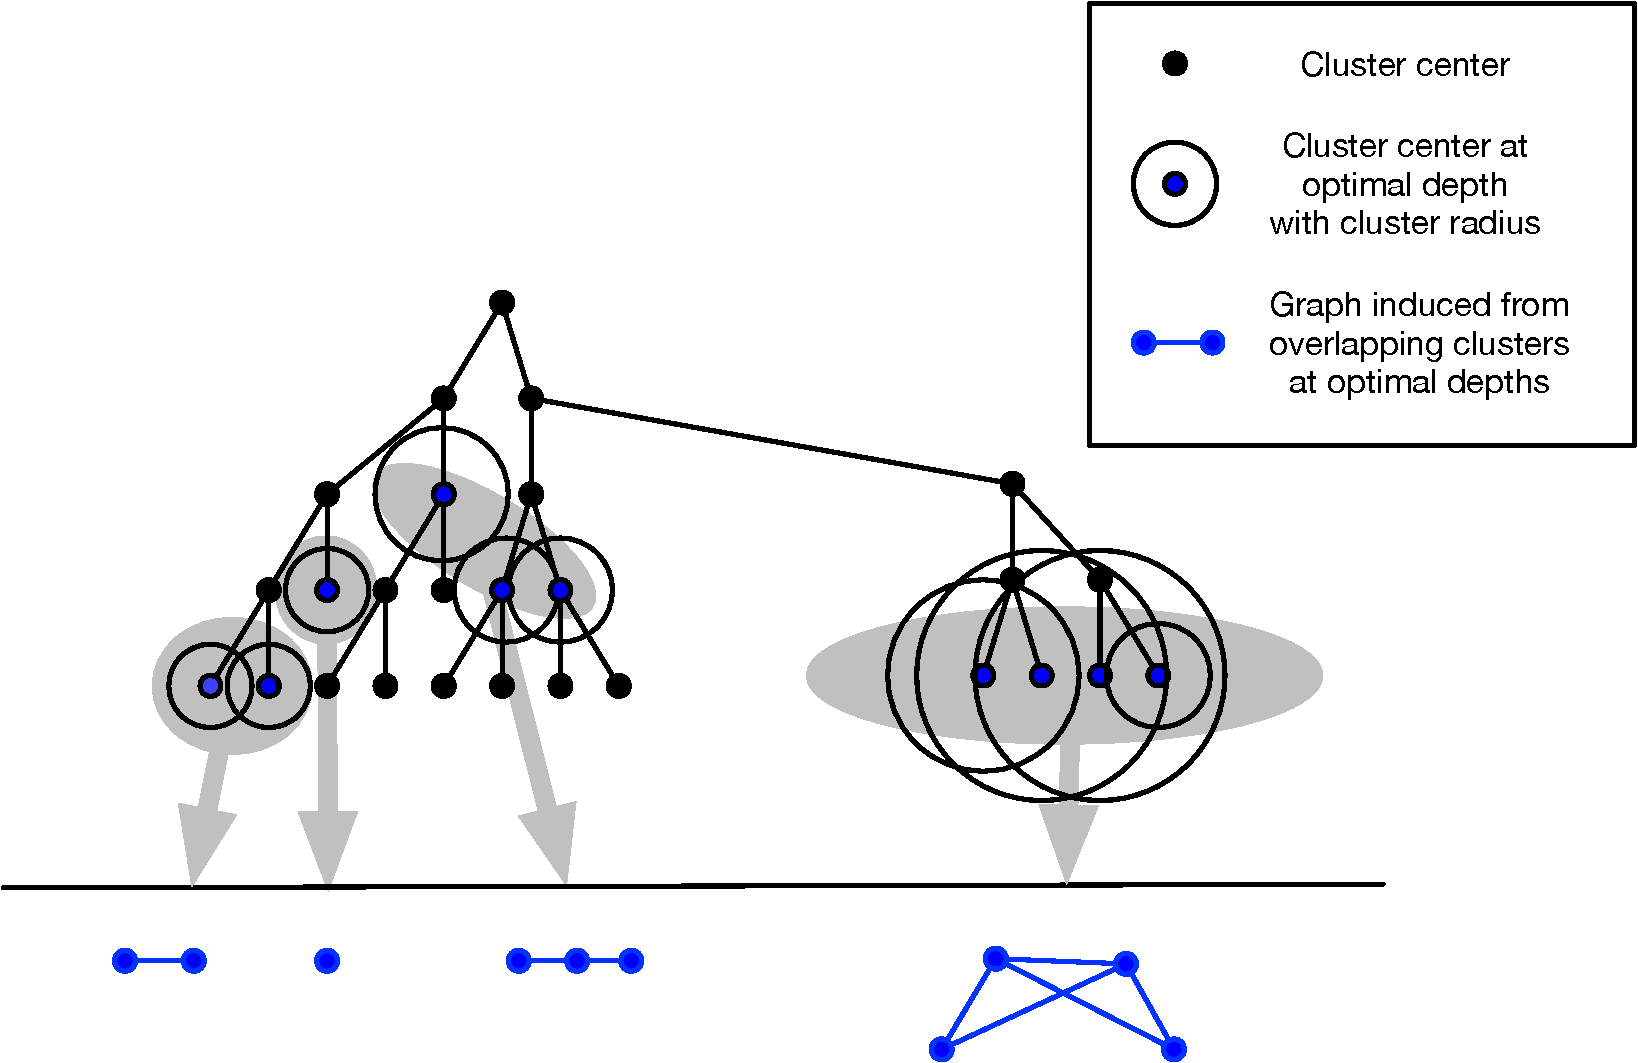
\includegraphics[width=3in]{images/tree-graph.pdf}
    \caption{Cartoon illustration of how CLAM induces a graph from a cluster tree.
        Dots in the tree represent cluster centers;
        blue dots represent cluster centers chosen as graph vertices.
        Circles around those centers represent the volume of a cluster (the radius is the distance from the center to the furthest point contained within that cluster).
        Gray arrows point to the induced subgraphs, which are indicated in blue below the horizontal line.}
    \label{fig:introduction:graph-generation}
\end{figure}

We test our methods on 24 real-world datasets.
The datasets span a wide variety of domains, each having a different quantity of anomalous data.
We consider several different definitions of outliers and anomalies: \textbf{distance-based}, examining several classical distance-based definitions of outliers, relying on CLAM's use of distance to cluster data; \textbf{density-based}, examining the cardinality of clusters, under the hypothesis that clusters with lower cardinality are more likely to contain outliers; \textbf{graph-based}, examining several graph-theoretic methods for anomaly detection, given graphs constructed from clusters.

Historically, clustering approaches have suffered from several problems.
The most common deficiencies are: the effective treatment of high dimensionality, the ability to interpret results, and the ability to scale to exponentially-growing datasets ~\cite{agrawal1998automatic}.
CLAM largely resolves these issues.

Na\"ively, distance-based approaches either require linear time in the cardinality of the data set, or quadratic time to build an index. 
CLAM builds an index in expected log-linear time and all CHAODA methods are sublinear in the cardinality of the dataset.

